\documentclass[border=10pt]{standalone}
\usepackage{pgfplots}
\usepgfplotslibrary{fillbetween}
\pgfplotsset{compat=1.18}
\begin{document}
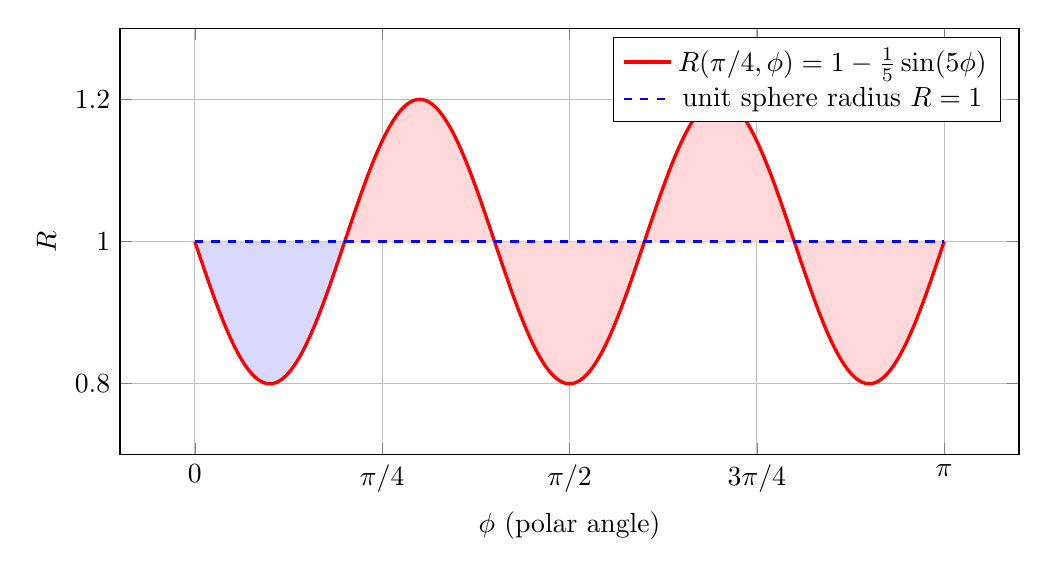
\begin{tikzpicture}
\begin{axis}[
    width=13cm,
    height=7cm,
    xlabel=$\phi$ (polar angle),
    ylabel=$R$,
    domain=0:180,
    samples=500,
    ymin=0.7,
    ymax=1.3,
    xtick={0,45,90,135,180},
    xticklabels={$0$,$\pi/4$,$\pi/2$,$3\pi/4$,$\pi$},
    grid=both,
    legend style={at={(0.98,0.98)}, anchor=north east},
]
\addplot[name path=A, very thick, red] {1-0.2*sin(5*x)};
\addlegendentry{$R(\pi/4,\phi)=1-\frac{1}{5}\sin(5\phi)$}
\addplot[name path=B, dashed, thick, blue] {1};
\addlegendentry{unit sphere radius $R=1$}
\addplot[red!15] fill between[of=A and B, split, every segment no 0/.style={blue!15}, every segment no 1/.style={red!15}];
\end{axis}
\end{tikzpicture}
\end{document}